\documentclass{IEEEcsmag}

\usepackage[colorlinks,urlcolor=blue,linkcolor=blue,citecolor=blue]{hyperref}
\expandafter\def\expandafter\UrlBreaks\expandafter{\UrlBreaks\do\/\do\*\do\-\do\~\do\'\do\"\do\-}
\usepackage{upmath,color}
\usepackage{graphicx}
\usepackage{booktabs}

\jvol{XX}
\jnum{XX}
\paper{8}
\jmonth{Month}
\jname{Computing in Science \& Engineering}
\jtitle{Computing in Science \& Engineering}
\pubyear{2026}

\setcounter{secnumdepth}{0}

\begin{document}

\sptitle{Feature Article: Research Software and Tools}

\title{From Code Repository to Research Infrastructure: Evaluating GitHub for Managing the Scientific Research Lifecycle}

\author{Telmo Miguel-Medina}
\affil{Electromechanical Engineering Department, University of Burgos, Burgos, 09001, Spain}

\markboth{FEATURE ARTICLE}{FEATURE ARTICLE}

\begin{abstract}\looseness-1
Research projects generate a long chain of interdependent artifacts --- questions, protocols, data, code, results, manuscripts --- that are usually managed across disconnected tools, with weak traceability of the process that produced them. This article asks how far GitHub's native, everyday features can serve as an integrated infrastructure for managing that process, not just for hosting its code. Combining a bibliometric map of 5{,}139 works with a structured review of the literature, I derive fifteen research-management requirements and score GitHub's native capabilities against each. GitHub meets thirteen of the fifteen requirements at a partial level or better, and seven directly, wherever research work looks like software engineering: tasks, review, communication, version history, documentation and automation. It falls short precisely where the literature itself is thinnest: tracking research questions, planning and decisions. A fifteen-component reference architecture and a reusable repository template package what works, and a year-long self-referential case study --- this project's own repository --- together with a retrospective check on an unrelated clinical machine-learning project, show the approach transfers. GitHub will not replace dedicated research infrastructure, but it can become the coordination and traceability layer that a fragmented research workflow currently lacks.
\end{abstract}

\maketitle

\chapteri{A} modern research project is not a single artifact but a chain of them: a question, a protocol, a literature corpus, data, analysis code, a computational environment, intermediate results, figures, a manuscript, and eventually released software and supplementary material. These objects evolve continuously, are touched by distributed and often multidisciplinary teams, and computational and data-intensive research keeps adding more of them while raising the cost of keeping them consistent.\textsuperscript{1}

In everyday practice, these artifacts and the work that produces them are scattered across disconnected systems --- email, cloud drives, spreadsheets, reference managers, statistical software, code repositories, task boards, manuscript editors. Each tool serves its own purpose well, but the layer that should coordinate them is largely missing. Reviews of research data management and of post-award grant management repeatedly link this fragmentation to weak decision traceability, incomplete process documentation, inconsistent versioning and low project visibility.\textsuperscript{2,3}

Two decades of work on scientific workflow systems, provenance, research data management and open-science platforms have produced solid evidence on stewarding research \emph{outputs} --- repositories, persistent identifiers, curation, dissemination.\textsuperscript{1,2,4} Managing the research \emph{process} itself --- planning, question formulation, decision tracking, cross-stage coordination --- has received far less systematic attention.\textsuperscript{5} The review literature is itself split into partly connected strands: workflow-system surveys that start from an executable pipeline and take the question and the plan behind it as given\textsuperscript{1}; provenance research that extends lineage tracking to data and computation but rarely reaches the upstream intellectual choices\textsuperscript{4}; data-management reviews centered on data as an output rather than the process that generated it\textsuperscript{2}; research-information-system reviews pitched at an institutional, reporting granularity\textsuperscript{6}; and open-science syntheses focused on transparency and incentives rather than day-to-day process management.\textsuperscript{7} A separate, mostly informal strand of guidance and case reports argues that Git and GitHub can carry collaborative, reproducible research in computational biology, ecology and the laboratory.\textsuperscript{8--10} This study cuts across all of these: it treats the research \emph{process} as the object to be managed and asks how far one widely available platform can cover the requirements each strand touches but none addresses as a whole.

GitHub already offers primitives for coordination, versioning, issue tracking, structured discussion, review and automation, and its footprint in the scholarly record is growing and measurable.\textsuperscript{11} But the evidence for using it as research infrastructure is case-based, and studies that mine GitHub as data caution that its use is heterogeneous and often shallow.\textsuperscript{12} Whether its native primitives can be organized into an infrastructure for managing the research process, and which parts of that process they can actually cover, had not been established on an evidentiary basis. This article answers that question directly: it does not claim GitHub replaces specialized research infrastructure, only that it can serve as the coordination and traceability layer research management currently lacks.

\section{HOW I STUDIED THIS}

The study combines three linked pieces of evidence, all built from openly available data and reproducible from a public repository. First, a bibliometric map: fifteen title-and-abstract queries against OpenAlex, spanning core process management, data management and open science, version control in research, and virtual research environments, filtered to 2008--2025 and cross-checked with five arXiv queries, produced a corpus of 5{,}139 works after de-duplication. An independent Scopus/Web-of-Science search sharing only 22\% of its DOIs with this corpus was inspected and found to add mostly low-precision tool citations rather than missed core literature, confirming the corpus as fit for purpose. Corpus concepts and abstracts were matched against an eleven-stage research-lifecycle lexicon (idea, question, planning, literature, methods, data, analysis, results, dissemination, outputs, governance) to produce a stage-coverage profile.

Second, a structured review of 52 secondary studies (reviews, surveys, syntheses) plus 15 primary studies of Git and GitHub use in research traced each documented literature problem to a management need and then to a derived requirement. Seventeen requirement rows were consolidated into fifteen research-management requirements (RM1--RM15), each with expected capabilities, lifecycle stage, supporting evidence and a rated importance; requirements rated high-importance but weak in literature attention were flagged as \emph{differentiators}. All coded decisions in the study were independently re-coded from the same source material; exact agreement was 96\%, leaving every figure reported here unchanged.

Third, GitHub's native functionality was catalogued as 68 capabilities across twelve feature groups (repositories, Markdown, Issues, Projects, Milestones, Labels, Discussions, Branches, Pull Requests, Actions, Releases, access control); marketplace and third-party apps were excluded, with one exception --- the GitHub--Zenodo release bridge, the de facto standard for persistent identification. Each requirement was then scored against the best support level GitHub's native functionality can reach with a reasonable implementation pattern, on a four-point rubric: Direct (a native feature meets it), Partial (met with an added convention), Limited (marginal), or Not supported.

The covered capabilities were then synthesized into a reference architecture and operationalized as a reusable, discipline-independent repository template. Finally, the framework was applied to managing this study itself --- a self-referential test in which the repository is the evidence --- and, retrospectively, to an unrelated, already-published clinical machine-learning project, to probe whether the pattern transfers across disciplines. Full query strings, coding sheets, the capability catalogue and every script that regenerates the figures and tables in this article are in the openly available study repository (see Acknowledgments).

\section{WHAT I FOUND}

\subsection{The literature is output-biased}

The 5{,}139-work corpus grows almost tenfold between 2008 and 2024, concentrated in computer science, library/information science and biomedicine, and spanning computer science, data science, knowledge management and the social sciences (Figure~\ref{fig:coword}). But its attention is markedly uneven: data management and analysis dominate (50.8\% and 41.9\% of the corpus), dissemination and coordination follow (24.4\% and 21.1\%), while idea and question formulation sit at the bottom (3.7\%), with provenance only slightly ahead (7.0\%). Seven of fifteen lifecycle stages --- idea, question, planning, ethics review, post-publication traceability, cross-stage coordination and governance --- are thinly covered, a bias the structured review of secondary studies reproduces independently.

\begin{figure}[t]
\centerline{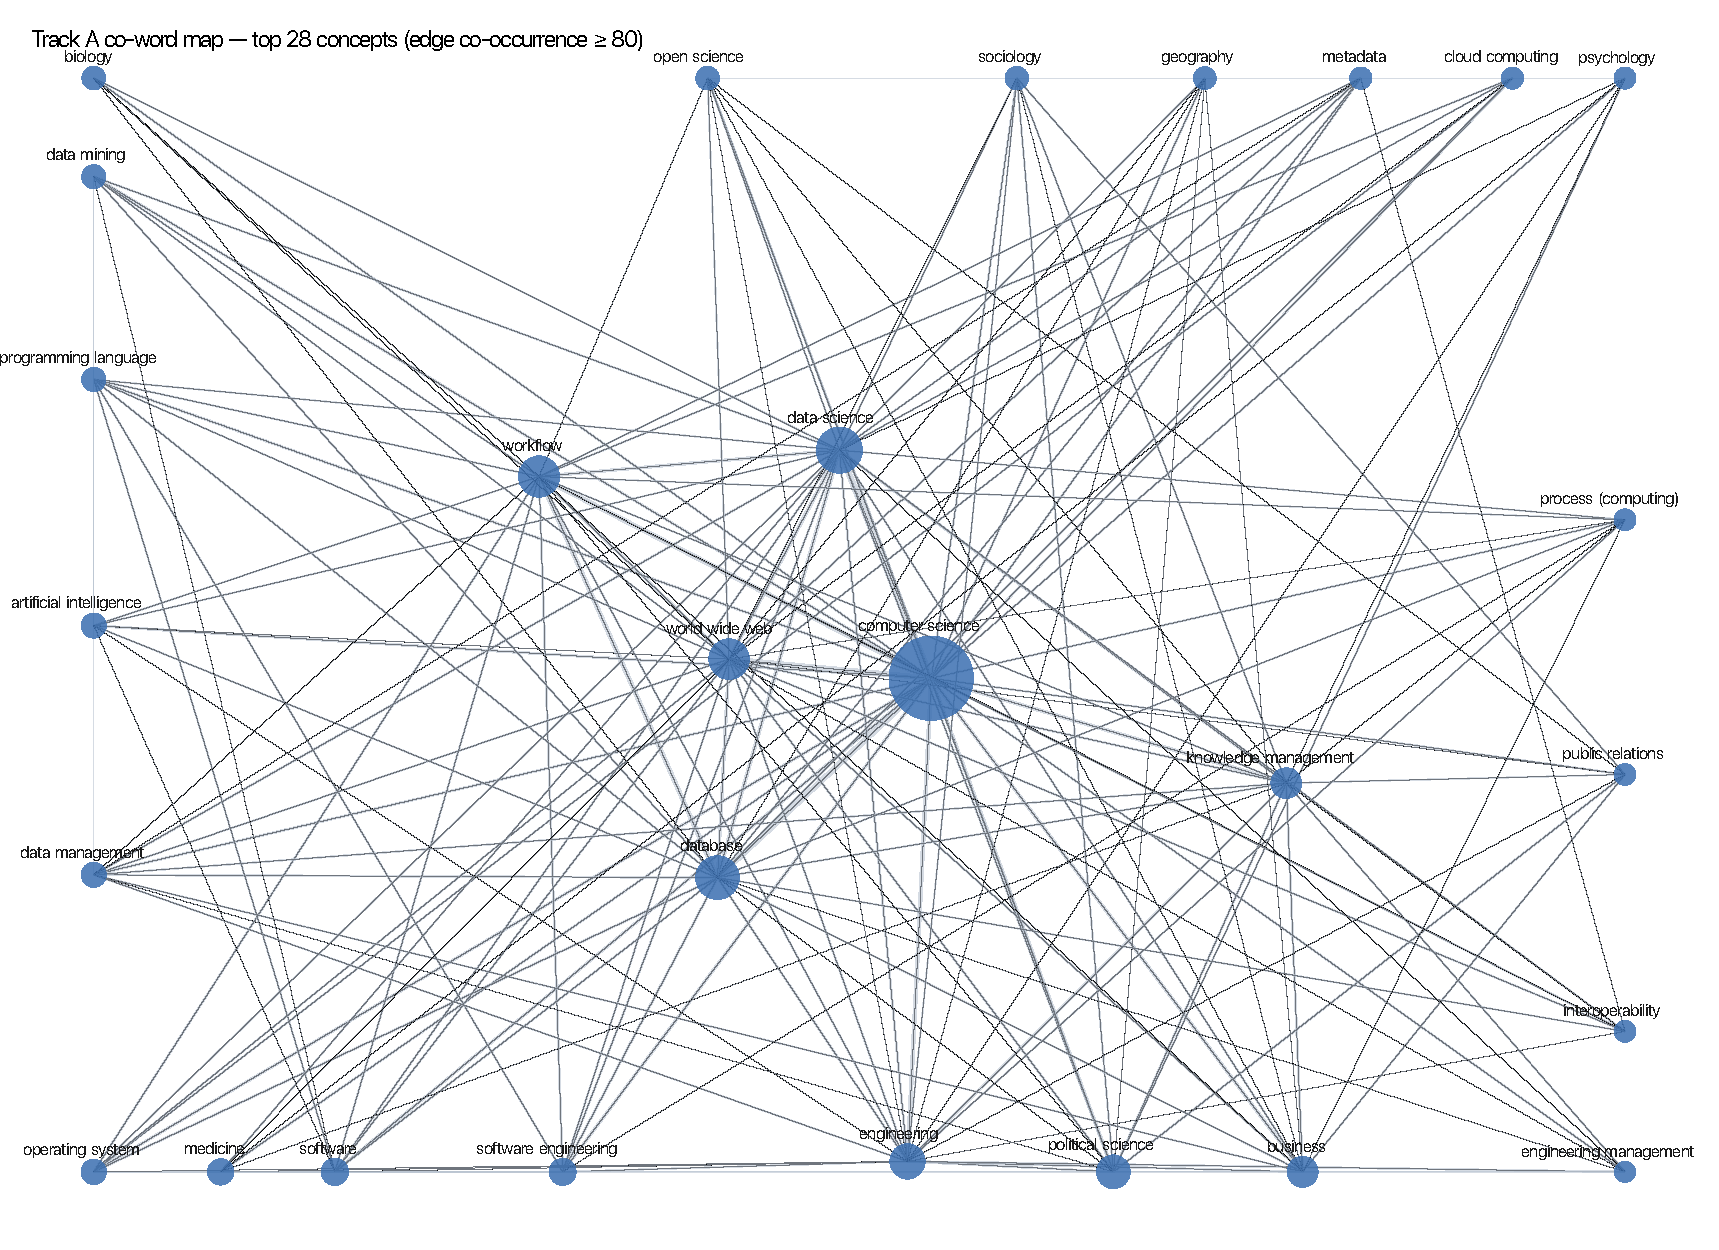
\includegraphics[width=18.5pc]{coword_map.pdf}}
\caption{Keyword co-occurrence map of the 5{,}139-work corpus. The field spans computer science, data science, information management and the social sciences, bridged by workflow, provenance and research-data-management terms --- but the upstream stages of the research process are largely absent from it.}\label{fig:coword}
\end{figure}

\subsection{GitHub covers execution well, planning poorly}

Fifteen research-management requirements emerged from the review, concentrated in traceability, documentation and collaboration. Three --- research planning, question management and decision traceability --- are rated highly important yet weakly served by the literature; these differentiators define the gap this study targets.

Table~\ref{tab:requirements} shows GitHub's native support for each. Thirteen of fifteen requirements are met at a Partial level or better, seven of them Direct, and none is entirely unsupported; average support is 2.43 out of 3 across the fourteen core requirements. Support is Direct wherever research work resembles software engineering: task management through Issues, a board and closing keywords that bind a task to the change that resolved it; documentation as version-controlled Markdown from day one; collaboration and communication through pull-request review and Discussions; version control as the platform's substrate; transparency as an inherent property of a public repository; and automation through Actions. Six requirements are only Partial, met by imposing a convention on a generic feature --- a Project field standing in for a research plan, a decision-record issue template standing in for a decision log, mandatory cross-referencing standing in for provenance linkage, pinned versions plus a re-run workflow standing in for reproducibility. Two requirements are Limited: no research-question object exists, so registering and tracking a question is entirely manual, and platform governance stops well short of institutional matters such as funding or workforce continuity. The differentiator requirements average 1.67 against 2.50 for the rest --- the same upstream gap the literature shows, reappearing independently in what GitHub actually supports. Five requirements --- large-data version control, cross-tool integration, reproducibility, persistent identification, and governance --- need external infrastructure GitHub cannot provide on its own.

\begin{table}[t]
\caption{The fifteen research-management requirements and GitHub's native support level: D = Direct, P = Partial, L = Limited. $^\star$ marks a differentiator (high importance, weak literature attention).}\label{tab:requirements}
\tablefont
\begin{tabular*}{17.5pc}{@{}p{175pt}p{40pt}<{\raggedright}@{}}
\toprule
Requirement& Support\\
\colrule
Research planning and roadmap$^\star$& P\\
Research question management$^\star$& L\\
Task management& D\\
Documentation& D\\
Decision traceability$^\star$& P\\
Collaboration and contribution tracking& D\\
Communication& D\\
Version control& D\\
Research artifact management and integration& P\\
Research provenance and artifact linkage& P\\
Transparency& D\\
Reproducibility support& P\\
Automation& D\\
Research output management and identification& P\\
Governance and sustainability& L\\
\botrule
\end{tabular*}
\end{table}

\subsection{A reusable architecture and template}

The covered capabilities organize into a fifteen-component, five-layer reference architecture (Figure~\ref{fig:arch}), in which GitHub acts as a coordination and traceability layer rather than a container: coordination (plan, activity tracker, question register, discussion space), record (documentation, decision log, linkage discipline, change history), production (artifact workspace, review, automation), release (release process, archival bridge, governance) and a cross-cutting transparency surface. One component --- \emph{linkage discipline}, the mandatory cross-referencing of every commit, pull request and issue --- and four named conventions are the framework's real contribution over a plain repository: they are what lift planning, question management, decision traceability and provenance from raw features toward research-usable support. Figure~\ref{fig:trace} shows the end-to-end traceability path this produces: a research question is referenced by the method that addresses it, whose branch and commits feed a reviewed pull request, whose result feeds the manuscript and a tagged, archived release. The architecture is operationalized as a 33-file, discipline-independent template --- a repository skeleton, issue forms, a pull-request checklist, Project field definitions, starter automation and a release checklist --- with every file mapped to the requirements it serves.

\begin{figure}[t]
\centerline{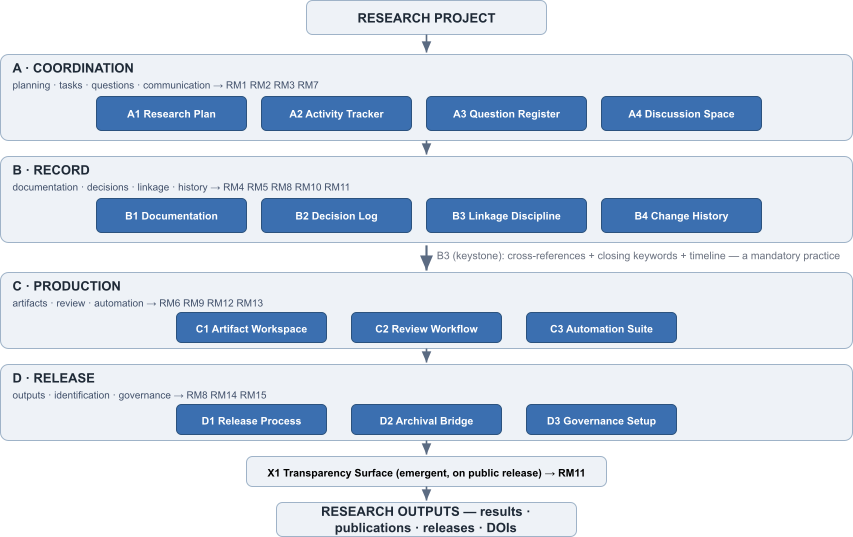
\includegraphics[width=18.5pc]{fig3_architecture.png}}
\caption{The GitHub-based reference architecture: five layers, fifteen components. GitHub is a coordination and traceability layer; large data, computational environments, persistent identifiers and institutional governance stay external and are linked by reference.}\label{fig:arch}
\end{figure}

\subsection{It works, at least once}

Applying the framework to this study itself, thirteen of fifteen components were exercised natively or partially; only the discussion space and the Zenodo archival bridge stayed planned. The documentation set (23 files) and a log of 26 decisions, each with context, rationale, alternatives and affected artifacts, were kept at full strength from the project's start at near-zero overhead. Once the repository was made public, its own backlog was pushed through one complete issue-to-release cycle, moving the coordination layer from configured to observed use. Scored across six dimensions --- coverage, traceability, documentation, organization, transparency and usability --- the framework reaches 1.86 out of 2 overall; usability is the weak point, at 1.50, driven by the Git, Markdown and YAML literacy the approach assumes, a real barrier outside computational fields.

\begin{figure}[t]
\centerline{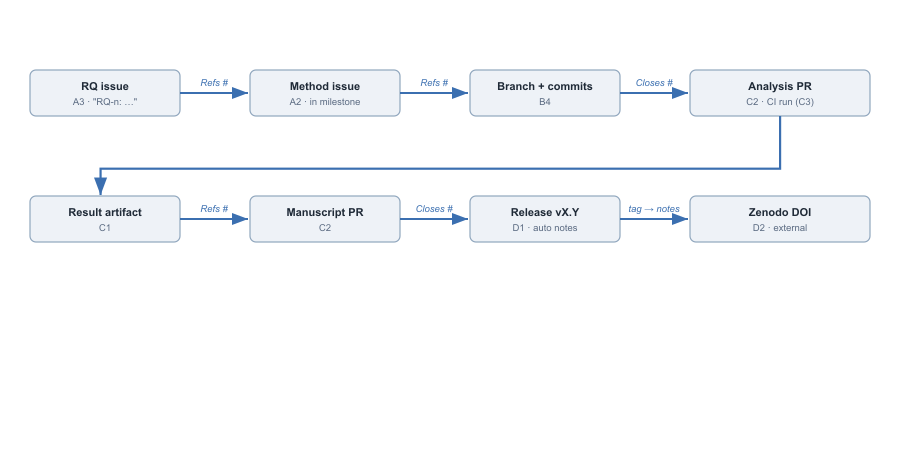
\includegraphics[width=18.5pc]{fig4_traceability.png}}
\caption{The traceability path produced by the linkage-discipline convention. Any node --- question, method, branch, pull request, result, manuscript, release --- is reachable from any other through recorded cross-references.}\label{fig:trace}
\end{figure}

Retrospectively instantiating the same template on an unrelated, already-published clinical machine-learning project (mortality prediction in cardiac surgery) reproduced the pattern: eight of fifteen requirements were served by a native template mechanism, three by an available-but-unexercised convention, and four --- restricted patient data, environment capture, full reproduction and institutional governance --- stayed outside the repository, in the same place the boundary fell for this project. The documentation, decision, version-control and output spine transferred directly across an unrelated discipline; only the constraint on the data changed, from ``large'' to ``access-restricted.''

\section{WHAT THIS MEANS}

The central result is a convergence reached by two independent routes: the literature under-serves idea and question formulation, planning and decision traceability, and GitHub supports those same requirements at 1.67 against 2.50 for the rest. Where research work can be expressed as files under version control, discrete tasks, branch-and-review changes and triggered automation, GitHub offers mature, purpose-built support, and it is genuinely low-cost --- a full plan of record and twenty-six logged decisions were produced with negligible overhead. Where the object of management is the evolving intellectual process itself --- the questions asked, the choices made and why --- GitHub offers only generic features on which a discipline must be imposed. Naming that discipline, as a linkage convention and three record conventions, is this framework's contribution; even so, the differentiator requirements stay Partial or Limited, so the framework maps the research-process-management gap rather than closing it.

Both the literature and GitHub's coverage are weakest at the earliest stages, because idea, question and planning work is deliberative and its ``artifacts'' are decisions rather than files. For an individual researcher or a small group, the practical path is to adopt the record layer first --- a version-controlled documentation folder, a decision log, disciplined commit messages --- since it delivers most of the traceability benefit at little cost; the Issue/Project/Pull-Request layer pays off once there are collaborators. The template lowers the setup cost of both, and its release and archival-bridge components hand a versioned, cross-referenced record to Zenodo, extending rather than replacing existing output-preservation tooling. Table~\ref{tab:comparison} contrasts this framework against the fragmented workflow it replaces.

\begin{table}[t]
\caption{A fragmented workflow versus the GitHub-based framework.}\label{tab:comparison}
\tablefont
\begin{tabular*}{17.5pc}{@{}p{68pt}<{\raggedright}p{115pt}<{\raggedright}@{}}
\toprule
Fragmented workflow& GitHub-based framework\\
\colrule
Tasks disconnected from the artifacts they produce& Issues, board and closing keywords bind task to commit to pull request\\[3pt]
Decisions in email and notes; rationale lost& Numbered decision log and decision issue, with rationale and affected artifacts\\[3pt]
Files renamed ``final''; no history& Git line-level history, diff, restore, tags\\[3pt]
Scattered documents; drift; no history& Version-controlled Markdown from project start\\[3pt]
No systematic link between question, data and result& Cross-references and timelines assemble the chain; release notes inherit it\\[3pt]
Visible only to the email loop& Public repository with status, activity log and changelog\\
\botrule
\end{tabular*}
\end{table}

Six limitations bound these findings. The framework maps the upstream gap without closing it. Its coordination layer was exercised once, end to end, under single-author conditions, so the collaborative value of review and parallel work on Issues, Projects and Pull Requests remains unproven. The evaluation is single-case and self-referential; an independent re-code of every coded decision agreed at 96\% but a second human rater was not available, and the retrospective second project shares this study's author. The primary corpus is OpenAlex plus arXiv, cross-checked but not replaced by Scopus/Web of Science. Roughly a third of GitHub's coverage rests on convention rather than native features. And GitHub is not a complete research infrastructure: persistent identifiers, computational environments, large datasets and institutional governance all stay external. A prospective, multi-author instantiation run from a project's start, and automated checks on the linkage-discipline convention itself, are the natural next steps.

\section{CONCLUSION}

GitHub can serve as an integrated coordination and traceability layer for a substantial part of the scientific research lifecycle. It supports thirteen of fifteen literature-derived requirements at Partial or better and seven directly, strong from execution to output and wherever research resembles software engineering, weak for the upstream traceability of questions, decisions and provenance --- the very requirements the literature also under-serves. A fifteen-component reference architecture, four conventions and a reusable template package what GitHub covers, and a year of self-referential use shows its documentation and version-control layer works at near-zero overhead while the collaborative value of its coordination layer still awaits a multi-author test. GitHub maps the research-process-management gap rather than closing it: not a replacement for research infrastructure, but the coordination and traceability layer a fragmented research workflow currently lacks.

\section{ACKNOWLEDGMENTS}
The study repository --- bibliographic corpus, coding sheets, requirement and mapping tables, reference architecture, reusable template and every script that regenerates this article's figures and tables --- is openly available at \url{https://github.com/telmomm/github-research-infrastructure-study} and archived on Zenodo, DOI \href{https://doi.org/10.5281/zenodo.22167500}{10.5281/zenodo.22167500}, with a companion dataset record at DOI \href{https://doi.org/10.5281/zenodo.22173525}{10.5281/zenodo.22173525}. The author declares no competing interests and received no specific funding for this work.

\def\refname{REFERENCES}

\begin{thebibliography}{1}

\bibitem{liew2016}
C. S. Liew, M. P. Atkinson, M. Galea, T. F. Ang, P. Martin, and J. I. van Hemert, ``Scientific workflows: Moving across paradigms,'' {\it ACM Comput. Surveys}, vol. 49, no. 4, pp. 1--39, 2016.

\bibitem{perrier2017}
L. Perrier et al., ``Research data management in academic institutions: A scoping review,'' {\it PLoS ONE}, vol. 12, no. 5, p. e0178261, 2017.

\bibitem{crane2023}
K. Crane, A. Blatch-Jones, and K. Fackrell, ``The post-award effort of managing and reporting on funded research: A scoping review,'' {\it F1000Research}, vol. 12, p. 863, 2023.

\bibitem{davidson2008}
S. B. Davidson and J. Freire, ``Provenance and scientific workflows: Challenges and opportunities,'' in {\it Proc. 2008 ACM SIGMOD Int. Conf. Manage. Data}, 2008, pp. 1345--1350.

\bibitem{cox2018}
A. Cox and W. Tam, ``A critical analysis of lifecycle models of the research process and research data management,'' {\it Aslib J. Inf. Manage.}, vol. 70, no. 2, pp. 142--157, 2018.

\bibitem{haris2026}
M. Haris, S. Auer, and M. Stocker, ``Research information systems and knowledge graphs: A review,'' {\it Front. Res. Metrics Anal.}, vol. 11, p. 1786866, 2026.

\bibitem{klebel2025}
T. Klebel, V. Traag, I. Grypari, L. Stoy, and T. Ross-Hellauer, ``The academic impact of Open Science: A scoping review,'' {\it R. Soc. Open Sci.}, vol. 12, no. 3, p. 241248, 2025.

\bibitem{blischak2016}
J. D. Blischak, E. R. Davenport, and G. Wilson, ``A quick introduction to version control with Git and GitHub,'' {\it PLoS Comput. Biol.}, vol. 12, no. 1, p. e1004668, 2016.

\bibitem{braga2023}
P. H. P. Braga et al., ``Not just for programmers: How GitHub can accelerate collaborative and reproducible research in ecology and evolution,'' {\it Methods Ecol. Evol.}, vol. 14, no. 6, pp. 1364--1380, 2023.

\bibitem{chen2025}
K. M. Chen, M. Toro-Moreno, and A. R. Subramaniam, ``GitHub enables collaborative and reproducible laboratory research,'' {\it PLoS Biol.}, vol. 23, no. 2, p. e3003029, 2025.

\bibitem{escamilla2022}
E. Escamilla, M. Klein, T. Cooper, V. Rampin, M. C. Weigle, and M. L. Nelson, ``The rise of GitHub in scholarly publications,'' in {\it Proc. Linking Theory Practice Digit. Libraries (TPDL 2022)}, 2022, pp. 187--200.

\bibitem{kalliamvakou2016}
E. Kalliamvakou, G. Gousios, K. Blincoe, L. Singer, D. M. German, and D. Damian, ``An in-depth study of the promises and perils of mining GitHub,'' {\it Empir. Softw. Eng.}, vol. 21, no. 5, pp. 2035--2071, 2016.

\end{thebibliography}

\begin{IEEEbiography}{Telmo Miguel-Medina}{\,}is with the Electromechanical Engineering Department, University of Burgos, Burgos, 09001, Spain. His research interests include research software engineering, open science infrastructure and reproducible computational research. Contact him at tmiguel@ubu.es.
\end{IEEEbiography}

\end{document}
